\documentclass[11pt]{standalone}
\usepackage{amssymb}
\usepackage{amsmath}
\usepackage[no-math]{fontspec}
\usepackage{unicode-math}
\usepackage{libertinus}
\usepackage{pgf,xcolor}
\usepackage{tikz}
\usetikzlibrary{arrows.meta, backgrounds, calc}
\usepackage{pgfplots}
\pgfplotsset{compat=newest}

\definecolor{my_darkgray}{HTML}{484949}
\definecolor{my_lightgray}{HTML}{F3F4F4}
\definecolor{my_darkblue}{HTML}{005A94}
\definecolor{my_lightblue}{HTML}{CCDEE9}
\definecolor{my_yellow}{HTML}{FFEC7F}
\definecolor{my_red}{HTML}{E60000}
\definecolor{my_orange}{HTML}{E87846}

\begin{document}
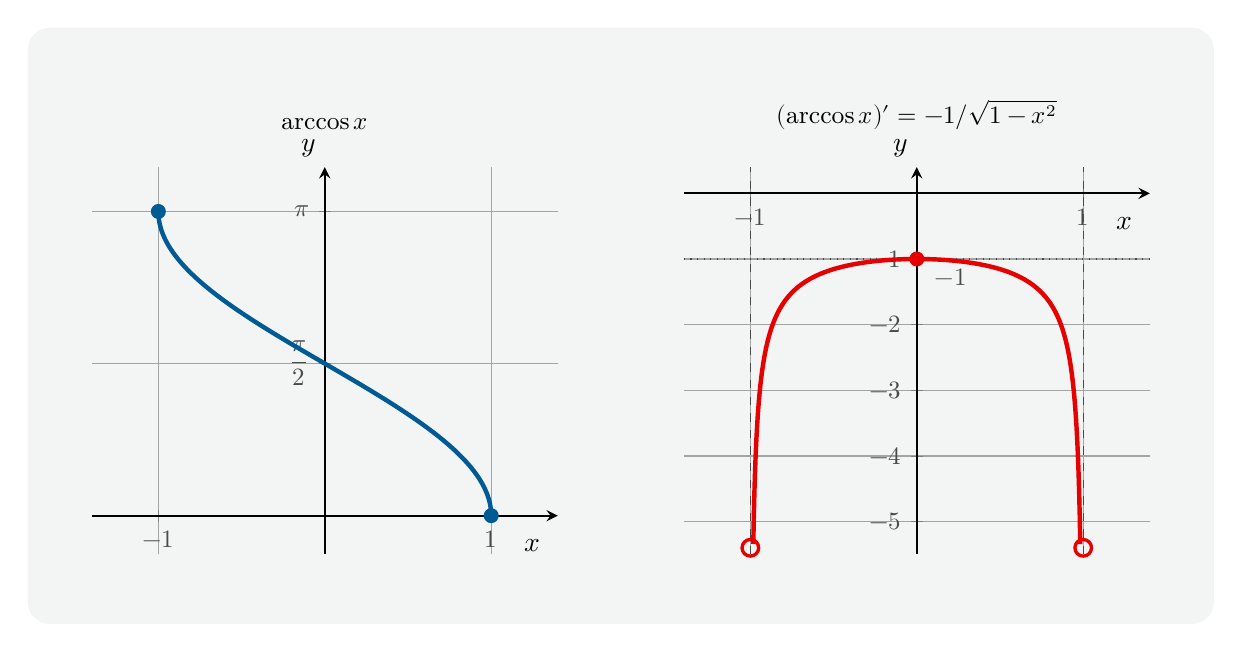
\begin{tikzpicture}[
    show background rectangle,
    background rectangle/.style={fill=my_lightgray, rounded corners=8pt},
    inner frame sep=0.8cm
]

% ── Left plot: arccos(x) ────────────────────────────────────────────────────
% Domain [-1, 1] closed; range [0, π].
% axis equal omitted: consistent with all other two-panel derivative figures.
\begin{axis}[
    name=left plot,
    axis lines = center,
    xlabel = {$x$},
    ylabel = {$y$},
    xlabel style = {at={(axis cs:1.25,0)}, anchor=north, yshift=-5pt},
    ylabel style = {anchor=south east},
    title = {$\arccos x$},
    title style = {font=\small, text=black, yshift=4pt},
    grid = both,
    grid style = {line width=0.3pt, draw=my_darkgray!30},
    major grid style = {line width=0.5pt, draw=my_darkgray!50},
    axis line style = {thick},
    xmin = -1.4, xmax = 1.4,
    ymin = -0.4, ymax = 3.6,
    xtick = {-1, 0, 1},
    ytick = {0, 1.5708, 3.14159},
    yticklabels = {$0$, $\dfrac{\pi}{2}$, $\pi$},
    yticklabel style = {font=\small, text=my_darkgray},
    xticklabel style = {font=\small, text=my_darkgray},
    width=7.5cm, height=6.5cm,
    clip=true,
]

\addplot[
    draw=my_darkblue,
    samples=500,
    ultra thick,
    domain=-1:1
]{ acos(x) * pi / 180 };

% Closed endpoints: domain [-1, 1] is a closed interval
\addplot[
    mark=*,
    mark size=2.5pt,
    only marks,
    draw=my_darkblue,
    fill=my_darkblue
] coordinates {(-1, 3.14159) (1, 0)};

\end{axis}

% ── Right plot: (arccos x)' = -1/sqrt(1 - x²) ──────────────────────────────
% Domain (-1, 1) open; diverges to -∞ as x → ±1.
% Maximum value is -1 at x = 0. The curve is the exact negative of (arcsin x)'.
% Domain kept away from ±1 to avoid sqrt(0); restrict y as safety net.
\begin{axis}[
    name=right plot,
    at={($(left plot.east)+(1.6cm,0)$)},
    anchor=west,
    axis lines = center,
    xlabel = {$x$},
    ylabel = {$y$},
    xlabel style = {at={(axis cs:1.25,0)}, anchor=north, yshift=-5pt},
    ylabel style = {anchor=south east},
    title = {$(\arccos x)' = -1/\sqrt{1-x^2}$},
    title style = {font=\small, text=black, yshift=4pt},
    grid = both,
    grid style = {line width=0.3pt, draw=my_darkgray!30},
    major grid style = {line width=0.5pt, draw=my_darkgray!50},
    % axis equal omitted: y range -5..0 vs x range ±1 – very different scales
    axis line style = {thick},
    xmin = -1.4, xmax = 1.4,
    ymin = -5.5, ymax = 0.4,
    xtick = {-1, 0, 1},
    ytick = {-5,-4,-3,-2,-1,0},
    yticklabel style = {
        /pgf/number format/fixed,
        /pgf/number format/precision=0,
        font=\small,
        text=my_darkgray
    },
    xticklabel style = {font=\small, text=my_darkgray},
    width=7.5cm, height=6.5cm,
    clip=true,
]

% Vertical asymptotes at x = ±1
\foreach \xa in {-1, 1}{
    \addplot[draw=my_darkgray, dashed, thin]
        coordinates {(\xa,-5.5) (\xa,0.4)};
}

% Dotted horizontal line at y = -1: maximum value at x = 0
\addplot[draw=my_darkgray, dotted, thin, domain=-1.4:1.4]{ -1 };
\node[anchor=north west, font=\small, text=my_darkgray]
    at (axis cs:0.05, -1) {$-1$};

% -1/sqrt(1-x²); restrict y to domain guards against blow-up near x = ±1
\addplot[
    draw=my_red,
    samples=600,
    ultra thick,
    domain=-0.9990:0.9990,
    restrict y to domain=-5.5:0
]{ -1 / sqrt(1 - x^2) };

% Mark the maximum (0, -1)
\addplot[
    mark=*,
    mark size=2.5pt,
    only marks,
    draw=my_red,
    fill=my_red
] coordinates {(0, -1)};

% Open circles at x = ±1: derivative undefined at the domain boundary
\addplot[
    mark=o,
    mark size=3pt,
    only marks,
    draw=my_red,
    fill=my_lightgray,
    line width=1.2pt
] coordinates {(-1, -5.4) (1, -5.4)};

\end{axis}

\end{tikzpicture}
\end{document}
